\chapter{Identifying Features using IPFs}
\label{chap:featureid}

\vspace{-\baselineskip}

%##################################################################################################
\section{Chapter Overview}
%##################################################################################################

In the previous chapter, we saw how to construct image partition forests from medical images using the watershed and waterfall transforms from mathematical morphology. This chapter now illustrates how these partition forests can be used when attempting to automatically identify features in abdominal CT scans.

Before looking at how to identify specific features in detail, I first describe a few techniques that can be used when constructing new feature identifiers. These range from simple node filtering to more novel methods such as \emph{stratified region growing}. I then describe two different classes of feature identifier: (1) those that identify features in 2D axial (X-Y) CT slices, as were implemented in my trial system, \emph{centipede}, and described in papers such as \cite{gvccimi08} and \cite{gvcispa09}, and (2) those that identify features in 3D CT volumes, as have been implemented in my final system, \emph{millipede}. (The approaches needed in the two cases have a certain amount in common, but differ in the details: for instance, when identifying the spine in 3D volumes, it is possible to use the property that it is a feature that extends through all the axial slices. This is quite powerful, since few 3D regions will do so. The same approach evidently cannot be used in 2D, since there is only one slice.)

This lays the foundation for Chapter~\ref{chap:validation}, in which the 3D identifiers used in \emph{millipede} will be validated against manually-produced, `gold-standard' results to quantify their accuracy. (The same will not be done for the 2D identifiers in \emph{centipede}, as they have now been superseded by their 3D counterparts; however, the quality of the 2D spine results was categorised in \cite{gvcispa09}.)

%##################################################################################################
\section{General Techniques}
%##################################################################################################

%Owing to the fact that different features in abdominal CT scans have widely differing properties, it is difficult to construct a framework to enable new feature identifiers to be constructed in anything like a mechanical way -- in general, a certain amount of invention is still required. However, there is nevertheless a great deal of low-level commonality between different identifiers -- while they may not share the same higher-level structure, they all make use of a number of general techniques, e.g.~filtering for regions that satisfy particular properties. This section thus describes these `building blocks', as a necessary precursor to presenting the actual identification algorithms.

%################################################
\subsection{Node Filtering}
%################################################

A basic feature identification technique is to filter all the (non-pixel) regions in the partition forest for those that satisfy a particular predicate (e.g.~those that have a mean grey value in a certain range). This is extremely simple to implement (see Listing~\ref{code:featureid-techniques-branchnodefiltering}), but can yield surprisingly good results when the features of interest are represented as individual regions in the forest. In terms of computational complexity, it is also an extremely efficient approach, being linear in the number of forest nodes.

%---
\begin{stulisting}[p]
\caption{Node Filtering Implementation}
\label{code:featureid-techniques-branchnodefiltering}
\lstinputlisting[style=Default]{featureid/featureid-techniques-branchnodefiltering.lst}
\end{stulisting}
%---

The predicate used to decide whether or not a node represents a specific feature can vary in its sophistication. Simple predicates that constrain region properties such as mean grey value, size and location often work surprisingly well, as will be seen when the 3D spine identifier is described later. A slightly more involved approach is to design the predicate using a \emph{Bayesian classifier} (this was used to design the 2D ribs identifier presented in \cite{gvccimi08}). For this, we first select a subset $X_1,\ldots,X_n$ of the region properties maintained for each branch node (for instance, we might select the four properties of \emph{area}, \emph{max grey value}, \emph{mean grey value} and \emph{elongatedness}). Given, for each property $X_i$, a distribution specifying the probability of each value of $X_i$ given that a node is or is not a specific feature -- that is, given $\mathbf{P}(X_i | \textit{Feature})$ for each $X_i$ -- it is possible to calculate a probability indicating the likelihood of a given node being an instance of that feature. Letting $\mathit{feature}$ denote $\mathit{Feature} = \mathit{true}$, $\neg \mathit{feature}$ denote $\mathit{Feature} = \mathit{false}$, and $x_i$ denote an observed value of $X_i$, this probability can be calculated using the equation:
%
\[
P(\mathit{feature}|x_1,\ldots,x_n) = \frac{P(\mathit{feature}) \displaystyle \prod_i P(x_i|\mathit{feature})}{\displaystyle \sum_{f \in \{\mathit{feature},\neg \mathit{feature}\}} \left[ P(f) \displaystyle \prod_i P(x_i|f) \right]}
\]
%
That is, given specific values of the chosen properties at a given node (for instance, an area of $250$, max grey value of $180$, mean grey value of $160$ and elongatedness of $2.5$), this equation will calculate a value giving us some indication of how likely it is that that node represents an instance of the feature in which we're interested. In order to use this to construct the required \emph{boolean} (i.e.~true or false) predicate, we simply choose a threshold probability above which regions qualify as instances of the feature in question. For instance, we could decide that a region represents a rib if the calculated probability of its being a rib (given its properties) is greater than $80\%$.

To make an approach based on Bayesian classification effective, it is important that suitable input probability distributions $\mathbf{P}(X_i | \textit{Feature})$ be available. These can either be defined empirically, or derived from a training set of images. For the 2D ribs identifier that will be described later, the distributions were defined empirically due to the lack of a sufficiently large set of data for training purposes -- the results produced were fairly good, but substantial trial-and-error development work was required. A learning approach is evidently preferable if sufficient data is available, although care must be taken not to over-fit to the training set. The approach taken for the 2D ribs identifier, that of manually defining input probabilities, did not appear to yield significant advantages over simpler, non-Bayesian techniques, and (despite the relatively good results obtained) is probably not a sensible basis for constructing future identifiers. A better method for identifying ribs is described in the section on 3D identifiers.

In many ways, node filtering in general can be seen as extending \emph{thresholding} from pixels to regions, taking advantage of the fact that regions, being larger, can have more interesting properties. (For example, rather than selecting pixels whose grey value is in a certain range, we can select regions whose mean grey value is in a certain range, that are of a reasonable size and that are (say) completely contained within the left-hand half of the image.) This intuitively suggests that it should be possible to lift other pixel-level segmentation algorithms to the region level; the next subsection does just that by developing what is effectively a region-level approach to region growing.

%################################################
\subsection{Stratified Region Growing}
\label{subsec:featureid-techniques-stratifiedregiongrowing}
%################################################

In \S\ref{subsec:background-segmentation-regiongrowing}, we saw a basic implementation of a single-seed region growing algorithm. This was pixel-based -- an individual pixel was chosen as the seed, and a region was then grown from it by choosing whether to add pixels adjacent to the existing region to the selection one at a time based on their pixel properties. However, the same technique can be lifted to the region level -- a region can be chosen as the seed, with surrounding regions then added to it or not based on their region properties (generally speaking, an aggregate of the properties of their pixels).

The idea of stratified region growing is to take this region-level region growing approach and adapt it to work with image partition forests, whose nodes represent regions of an image. Rather than starting from a single seed, stratified region growing first filters the forest's branch nodes for (potentially) multiple seeds in multiple layers of the forest. It then grows a region from each seed in the adjacency graph of the seed's layer. Finally, the regions grown are unioned (e.g.~using a partition forest selection, as it is convenient to do so) to produce the result. See Listing~\ref{code:featureid-techniques-stratifiedregiongrowing} for pseudo-code, and Figure~\ref{?} for an illustration of the process.

%---
\begin{stulisting}[p]
\caption{Stratified Region Growing Implementation}
\label{code:featureid-techniques-stratifiedregiongrowing}
\lstinputlisting[style=Default]{featureid/featureid-techniques-stratifiedregiongrowing.lst}
\end{stulisting}
%---

Stratified region growing is interesting because the regions for the seeds are grown at different scales. One problem with growing regions only at the pixel level is that minor changes to the image (for instance, lowering the grey value of a small number of pixels) can dramatically affect the result. Conversely, running the process only at the level of large regions can result in fine detail being missed -- it can even be impossible to obtain a sensible result if the large regions don't match the feature. If used carefully, stratified region growing (and indeed other methods which operate at more than one scale) can mitigate these problems at least some of the time.

It should be noted that there is room for a certain amount of variation in how the technique is used in practice. For instance, the 2D spine identifier that will be described later (and was originally presented in \cite{gvcispa09}) `validates' the regions grown from individual seeds before adding them to the result. The precise workings of the algorithm itself are also open to modification -- for example, the 2D spine identifier as originally defined doesn't grow regions from seeds that have already been visited during region growing from an earlier seed (though that approach does mean that an ordering must be imposed on the seeds, which makes it difficult to parallelize). For the purposes of this dissertation, however, stratified region growing will refer specifically to the implementation described here, unless otherwise stated (in particular, the 2D spine identifier will be described explicitly as a variant of this approach).

%################################################
\subsection{Conditional Morphology}
%################################################

As originally mentioned in \S\ref{subsec:background-segmentation-morphology}, there is far more to the field of mathematical morphology than image segmentation techniques such as the watershed transform. Of particular interest for feature identification work are morphological operators such as \emph{dilation}, \emph{erosion}, \emph{opening} and \emph{closing}; closing in particular is a useful tool for filling in holes in identified features (such as those produced by region growing). The canonical formulation of these processes is as operators on binary or grey-scale images, but of more relevance for our purposes is their adaptation to graphs (e.g.~see \cite{heijmans92a}), since the partition forest is essentially a graph hierarchy. We therefore examine only graph-based morphological operators here -- interested readers are encouraged to consult \cite{gonzalez02} for a description of their more conventional, image-based equivalents.

Image-based morphological operators are often defined in terms of a tiny shape called a \emph{structuring element}, for example a $3 \times 3$ square, but non-structured versions are also possible. For graphs, non-structured operators were studied first, with structured operators defined in terms of \emph{structuring graphs} (the graph-based equivalent of structuring elements) introduced later in \cite{heijmans92a}. However, for the feature identification algorithms described in this chapter, the non-structured operators were considered appropriate. As will be described later, the versions we use in practice are actually parameterised by user-specified conditions that control how the process works, but the non-conditional versions will be presented first for the purposes of explication.

%~~~~~~~~~~~~~~~~~~~~~~~~~~~~~~~~~~~~~~~~~~~~~~~~
\subsubsection{Non-Structured Dilation}
%~~~~~~~~~~~~~~~~~~~~~~~~~~~~~~~~~~~~~~~~~~~~~~~~

The first morphological graph operator we will examine, then, is non-structured dilation. Given an undirected graph $G = (V,E)$ and a set $S \subseteq V$ of selected nodes, the \emph{elementary} non-structured dilation of $S$, which we will write as $\delta(S)$ to follow the convention given in \cite{heijmans92a}, is defined as:
%
\[
\delta(S) = S \cup \{v \in V \; | \; \exists u \in S \cdot \{v,u\} \in E\}
\]
%
In other words, performing an elementary non-structured dilation on a set $S$ of selected nodes means augmenting the selection with those nodes that are directly adjacent to nodes in $S$. This is illustrated in Figure~\ref{fig:featureid-techniques-dilation}.

%---
\begin{stusubfig}{p}
	\subfigure[The initial selection]
	{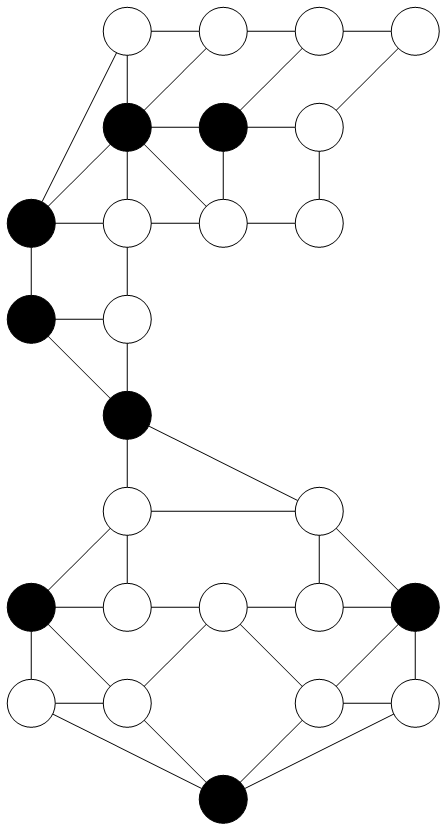
\includegraphics[height=8cm]{featureid/featureid-techniques-dilation-a.png}}%
	%
	\hspace{12mm}%
	%
	\subfigure[After dilating]
	{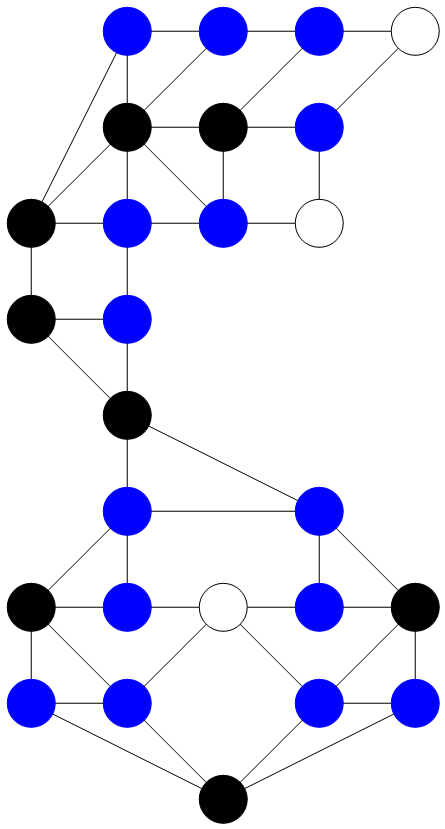
\includegraphics[height=8cm]{featureid/featureid-techniques-dilation-b.png}}%
\caption{Elementary non-structured morphological dilation on graphs: the black nodes are those initially selected and the blue nodes are those added by the dilation.}
\label{fig:featureid-techniques-dilation}
\end{stusubfig}
%---

As described in \cite{heijmans92a}, several elementary non-structured dilations can also be chained together to give the size $n$ non-structured dilation of $S$:
%
\[
\delta^{(n)}(S) = (\underbrace{\delta \bullet \delta \bullet \cdots \bullet \delta}_{n \mbox{ times}})(S)
\]
%
As with the image-based dilation described in \cite{gonzalez02}, graph-based dilation is useful for gap bridging and, to a certain extent, hole filling. Dilations of larger sizes can be used to bridge wider gaps or fill larger holes. However, because it works by expanding boundaries, dilation makes the selection as a whole grow -- whilst it can be used to fill internal holes, it achieves this in a way that drastically changes the size of the overall selection. The closing operator (described later) avoids this problem by first performing a dilation, and then eroding the result. This yields much better results for hole filling.

%~~~~~~~~~~~~~~~~~~~~~~~~~~~~~~~~~~~~~~~~~~~~~~~~
\subsubsection{Non-Structured Erosion}
%~~~~~~~~~~~~~~~~~~~~~~~~~~~~~~~~~~~~~~~~~~~~~~~~

The counterpart of non-structured dilation is non-structured erosion. Given an undirected graph and set $S$ as defined above, the \emph{elementary} non-structured erosion of $S$ is:
%
\[
\epsilon(S) = \{v \in S \; | \; \not\exists u \in V \; \backslash \; S \cdot \{v,u\} \in E\}
\]
%
That is, performing an elementary non-structured erosion on $S$ means removing all the boundary nodes from $S$. This is illustrated in Figure~\ref{fig:featureid-techniques-erosion}.

%---
\begin{stusubfig}{p}
	\subfigure[The initial selection]
	{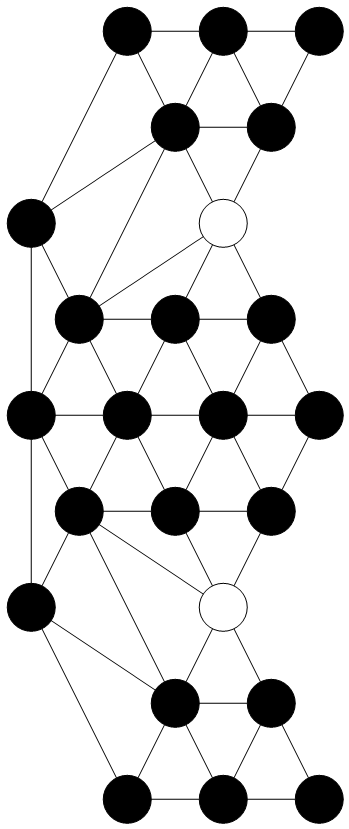
\includegraphics[height=8cm]{featureid/featureid-techniques-erosion-a.png}\hspace{12mm}}%
	%
	\hspace{4mm}%
	%
	\subfigure[After eroding]
	{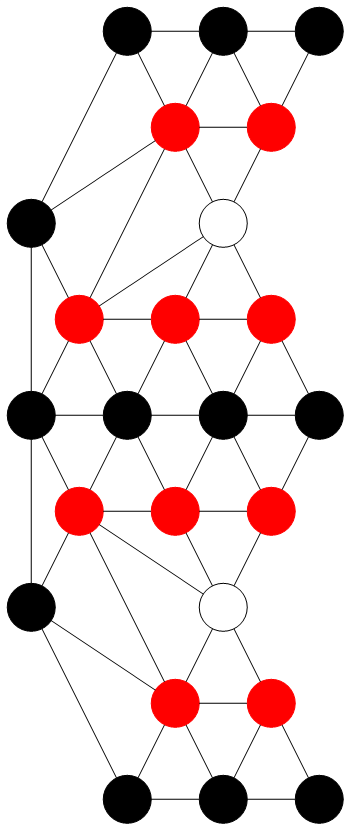
\includegraphics[height=8cm]{featureid/featureid-techniques-erosion-b.png}}%
\caption{Elementary non-structured morphological erosion on graphs: the black nodes are those initially selected and the red nodes are those removed by the erosion.}
\label{fig:featureid-techniques-erosion}
\end{stusubfig}
%---

As with dilation, several elementary non-structured erosions can be chained together to give the size $n$ non-structured erosion of $S$:
%
\[
\epsilon^{(n)}(S) = (\underbrace{\epsilon \bullet \epsilon \bullet \cdots \bullet \epsilon}_{n \mbox{ times}})(S)
\]
%
As with the image-based erosion described in \cite{gonzalez02}, graph-based erosion is a useful tool to remove small, irrelevant pieces from the selection. Erosions of larger sizes can be used to remove larger pieces. As with dilation, however, erosion seriously affects the size of the overall selection. Whilst this has its uses, there are applications for which the goal is to improve the existing selection without changing its extent too much. For such applications, the higher-level opening and closing operators described next tend to be more useful than dilation and erosion.

%~~~~~~~~~~~~~~~~~~~~~~~~~~~~~~~~~~~~~~~~~~~~~~~~
\subsubsection{Non-Structured Opening}
%~~~~~~~~~~~~~~~~~~~~~~~~~~~~~~~~~~~~~~~~~~~~~~~~

The non-structured opening operator of size $n$ first erodes $S$ and then dilates the result:
%
\[
\sigma^{(n)} = \delta^{(n)} \bullet \epsilon^{(n)}
\]
%
The intuition is that this starts by removing small, irrelevant pieces and making larger pieces smaller, and then roughly restores the larger pieces to their original size again (this isn't strictly true, since information is lost when the larger pieces are eroded, but it is a useful way of thinking about it). The way opening works is illustrated in Figure~\ref{?}.

As with the image-based opening described in \cite{gonzalez02}, graph-based opening is useful for things like removing narrow connections between larger pieces of the selection. Somewhat wider connections can be removed by opening with a larger size, but this runs the risk of adversely affecting the rest of the selection.

%~~~~~~~~~~~~~~~~~~~~~~~~~~~~~~~~~~~~~~~~~~~~~~~~
\subsubsection{Non-Structured Closing}
%~~~~~~~~~~~~~~~~~~~~~~~~~~~~~~~~~~~~~~~~~~~~~~~~

The counterpart of non-structured opening is non-structured closing. The non-structured closing operator of size $n$ first dilates $S$ and then erodes the result:
%
\[
\kappa^{(n)} = \epsilon^{(n)} \bullet \delta^{(n)}
\]
%
The intuition is that this starts by expanding the boundaries of the selection (including internal boundaries, which fills in holes) and then erodes the remaining boundaries (which we hope are the outer ones) to return the selection to something like its original size (again, this isn't strictly true, but it gives a rough guide to what is happening). The way closing works is illustrated in Figure~\ref{?}.

Closing is a good tool for filling in holes. Larger holes can be filled in by closing with a larger size, but care must again be taken to avoid damaging the rest of the selection.

%~~~~~~~~~~~~~~~~~~~~~~~~~~~~~~~~~~~~~~~~~~~~~~~~
\subsubsection{Conditioning}
%~~~~~~~~~~~~~~~~~~~~~~~~~~~~~~~~~~~~~~~~~~~~~~~~

The operators as described thus far are useful, but can be quite blunt instruments. For example, dilation takes no account of what is beyond the boundaries when expanding the selection, so it can be difficult to avoid damaging the outer boundary of the selection when trying to fill holes (see Figure~\ref{?}(b)). Better results (see Figure~\ref{?}(c)) can be obtained by allowing the user to specify \emph{conditions} that determine when to allow dilation into or erosion of a graph node, e.g.~that a node beyond the boundary should only be added to the selection during dilation if its mean grey value lies in a particular range. This approach is known (for obvious reasons) as \emph{conditional morphology}; implementations of the conditional morphological operators are shown in Listing~\ref{code:featureid-techniques-conditionalmorphology}. These are the operators that we will use in practice when implementing the 3D feature identifiers described later.

%---
\begin{stulisting}[p]
\caption{Implementation of Conditional Morphological Operators}
\label{code:featureid-techniques-conditionalmorphology}
\lstinputlisting[style=Default]{featureid/featureid-techniques-conditionalmorphology.lst}
\end{stulisting}
%---

%################################################
\subsection{Connected Component Analysis}
%################################################

When identifying features, it is sometimes useful to work with the connected components of an intermediate feature selection. For instance, it will be seen later that the 3D ribs identifier first uses stratified region growing to produce an initial selection for the ribs, and then post-processes it, examining each connected component to see how rib-like it is.

Given a set of nodes in a particular layer of the partition forest, it is clearly a simple process to determine their connected components for such processing (see Appendix~\ref{chap:appendixpf} for pseudo-code). However, partition forest selections have a representation that is multi-layer (see Chapter~\ref{chap:ipfs}) -- it is therefore necessary to view the selection at a particular layer so as to ensure that all the nodes being dealt with are at the same level, namely the lowest layer containing a selected node. As explained when it was described, the view at layer algorithm splits higher-level nodes into their descendants in the chosen layer, whilst leaving lower-level nodes alone. The result in this case is thus a set of nodes in a single layer. The connected components of these nodes (and the properties of each component) can then be easily determined.

\afterpage{\clearpage}
\newpage

%##################################################################################################
\section{Feature Identification in Axial Slices}
%##################################################################################################

%################################################
\subsection{Overview}
%################################################

Having examined some general feature identification techniques, we now turn our attention to ways of identifying specific features. The first feature identifiers we will look at were designed to identify the ribs and spine in 2D, axial (X-Y) CT slices, and implemented in the trial system, \emph{centipede}. The identifiers implemented in the final system, \emph{millipede}, which seek to identify a much wider range of features in 3D CT volumes, will be presented subsequently.

%################################################
\subsection{Ribs Identification}
%################################################

The 2D ribs identifier, a sample result of which was originally presented in \cite{gvccimi08}, works as follows:

\begin{enumerate}

\item Initially, a Bayesian classifier is used to determine the likelihood (in some sense) of a region in the forest being a rib.
\item Then, the \emph{saliency} of the region (that is, the minimum difference in mean grey value between the region and its neighbours) is evaluated. Regions whose saliency is less than $50$ (a value determined empirically, bearing in mind that the grey values in the image range between $0$ and $255$) are considered insufficiently salient (i.e.~they do not `stand out' enough relative to their neighbours) and are discarded.
\item Finally, if the region survives and has a greater than $80\%$ likelihood of being a rib, it is added to the final result.

\end{enumerate}

\noindent The Bayesian classifier itself is based on four properties of the regions involved: their \emph{area}, \emph{elongatedness}, \emph{maximum grey value} and \emph{mean grey value}. As described in \cite{gvccimi08}, rib regions can intuitively be identified in axial slices by their relatively small (cross-sectional) area, high maximum grey value, relatively high mean grey value and noticeable, but not extreme elongatedness. In more practical terms, these qualitative descriptions can be turned into quantitative distributions by representing them as \emph{fuzzy sets} (a technique employed in a similar context in \cite{lee03}). A fuzzy set is a generalization of the set concept that allows objects to be only partly members of a set. Fuzzy sets are generally represented using a membership function $m$ that specifies the degree of membership of each relevant object as a number between $0$ and $1$. Thus, $m(e) = 0$ means that $e$ is in no way a member of the fuzzy set, $m(e) = 1$ means that it is entirely in the fuzzy set, and $m(e) = 0.7$ (for example) means that it is $70\%$ in the fuzzy set and $30\%$ not in it.

In the present case, we can (for example) define the fuzzy set of regions that have the correct area to be a rib, and use it as our probability distribution $\mathbf{P}(\mathit{Area} | \mathit{rib})$. By observing rib-like regions in multiple image series, we can determine that most ribs in $512 \times 512$ axial images have areas in the $[180,350)$ pixel range, with some outliers in the $[70,180)$ and $[350,400)$ pixel ranges. From this, we can then simply construct the piecewise linear membership function shown in Figure~\ref{fig:featureid-2d-ribsidentification-areamembership}, which makes regions with pixel areas in $[180,350)$ full members of the fuzzy set, with membership tailing off based on distance from this central range (regions with areas $< 70$ or $\ge 400$ are considered either too small or too large to be ribs, respectively). A similar membership function can be empirically determined for each of the other properties -- in each case, we use this as our probability distribution $\mathbf{P}(\mathit{Property} | \mathit{rib})$. By contrast, when defining the $\mathbf{P}(\mathit{Property} | \neg\mathit{rib})$ probability distributions for the four properties, constant probabilities were in practice found to work well.

%---
\begin{stulisting}[p]
\caption{Ribs Identification in 2D}
\label{code:featureid-2d-ribsidentification}
\lstinputlisting[style=Default]{featureid/featureid-2d-ribsidentification.lst}
\end{stulisting}
%---

%---
\stufigex{height=7cm}{featureid/featureid-2d-ribsidentification-areamembership.png}{The membership function for the fuzzy set of regions that have the correct area to be a rib in 2D axial slices}{fig:featureid-2d-ribsidentification-areamembership}{p}
%---

%---
\begin{stusubfig}{p}
	\subfigure[]
	{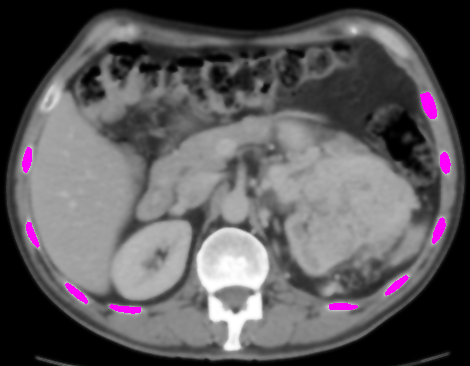
\includegraphics[width=.4\linewidth]{featureid/featureid-2d-ribsidentification-example-a.png}}%
	%
	\hspace{4mm}%
	%
	\subfigure[]
	{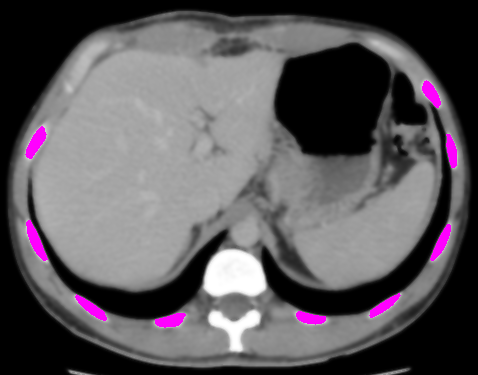
\includegraphics[width=.4\linewidth]{featureid/featureid-2d-ribsidentification-example-b.png}}%
	%
	\hspace{4mm}%
	%
	\subfigure[]
	{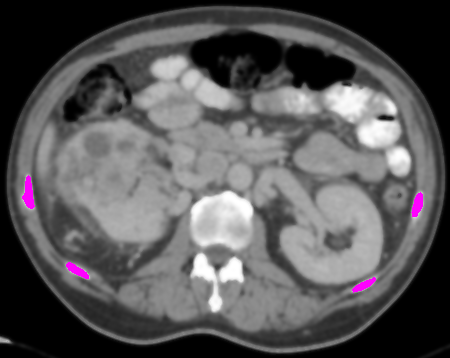
\includegraphics[width=.4\linewidth]{featureid/featureid-2d-ribsidentification-example-c.png}}%
	%
	\hspace{4mm}%
	%
	\subfigure[]
	{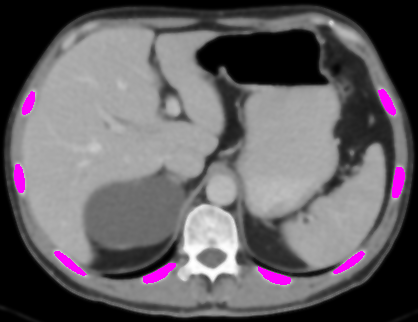
\includegraphics[width=.4\linewidth]{featureid/featureid-2d-ribsidentification-example-d.png}}%
\caption{Example results of the 2D ribs identifier on images from several different series}
\label{fig:featureid-2d-ribsidentification-example}
\end{stusubfig}
%---

Pseudo-code for the ribs identifier is shown in Listing~\ref{code:featureid-2d-ribsidentification}. As illustrated in Figure~\ref{fig:featureid-2d-ribsidentification-example}, this approach can identify ribs quite well (although some darker ribs, such as that in (a), can be missed). However, it is evidently somewhat ad-hoc, in that the probability distributions were customised by hand -- a better approach would have been to manually identify the ribs in a training set of image series, and then automatically construct the probability distributions from the marked and unmarked regions. At the time of designing the identifier, this approach was not advisable due to the amount of data I had available at the time (only $3$ series) -- there would have been a serious risk of overfitting to a small number of images. When more data is available, automatically-constructed probability distributions are almost certainly the better option. In practice, however, a much more effective way of improving the identification of the ribs is simply to work with 3D volumes rather than 2D axial slices -- this was the approach used in \emph{millipede}, which will be described in \S\ref{subsec:featureid-3d-ribsidentification}.

\newpage

%################################################
\subsection{Spine Identification}
%################################################

The 2D spine identifier, originally described in \cite{gvcispa09}, uses a variant of stratified region growing to extract a preliminary spine feature from the image, and then post-processes it to identify the final vertebra. The outline of the algorithm is as it was described in the paper:

%-
\begin{enumerate}

\item \textbf{Seed Finding}. Filter for branch nodes that satisfy a user-specified \emph{seed criterion}.
\item \textbf{Region Growing}. Determine the \emph{preliminary feature} (which will be represented as a partition forest selection) by growing regions from the various seeds.

%--
\begin{enumerate}

\item Construct a map to indicate whether or not each seed has yet been visited during the region growing process (each seed is initially marked as unvisited).
\item For each seed:

%---
\begin{enumerate}

\item If the seed has not already been visited, identify a \emph{potential partial feature} for it by growing a region from it in the adjacency graph for its layer. The region growing process is (as usual) controlled by a user-specified \emph{growing criterion}.
\item If the potential partial feature satisfies a user-specified \emph{validation criterion}, add its regions to the preliminary feature.
\item Mark any seeds that were reached from the current seed as having been visited.

\end{enumerate}
%---

\end{enumerate}
%--

\item \textbf{Post-Processing}. Remove any regions that were undesirably added by the region growing process (the regions to be removed are chosen via the means of a user-specified \emph{removal criterion}).

%--
\begin{enumerate}

\item For each region in the representation of the partition forest selection for the preliminary feature:

%---
\begin{enumerate}

\item If the region satisfies the removal criterion, remove it from the selection (using the node deselection algorithm for partition forest selections).
\item Otherwise, recurse on its (branch node) children in the forest (if any).

\end{enumerate}
%---

\end{enumerate}
%--

\end{enumerate}
%-

\noindent Pseudo-code for this process is shown in Listing~\ref{code:featureid-2d-spineidentification}, and Figure~\ref{fig:featureid-2d-spineidentification} provides a graphical overview of how it works. It will be observed that the first two steps of this algorithm essentially implement a variation of the stratified region growing approach described in \S\ref{subsec:featureid-techniques-stratifiedregiongrowing}. The significant differences are that (a) the approach here keeps track of which seeds have been visited whilst growing regions from other seeds, and avoids growing a region from a seed if it has already been seen, and (b) the region grown from each seed is validated before being added to the preliminary feature. When the algorithm was originally devised, the first of these tweaks was intended to avoid growing similar regions more than once, whilst the second was intended as an alternative to performing connected component analysis on the preliminary feature. With the benefit of hindsight, it is potentially better to implement a simpler stratified region growing approach that avoids these complications (and is easier to parallelize), and then perform connected component analysis on the results during post-processing. However, the original approach is described here so as not to affect the validity of the presented results.

%---
\begin{stulisting}[p]
\caption{Spine Identification in 2D : Main Algorithm}
\label{code:featureid-2d-spineidentification}
\lstinputlisting[style=Default]{featureid/featureid-2d-spineidentification.lst}
\end{stulisting}
%---

%~~~~~~~~~~~~~~~~~~~~~~~~~~~~~~~~~~~~~~~~~~~~~~~~
\subsubsection{Seed Finding}
%~~~~~~~~~~~~~~~~~~~~~~~~~~~~~~~~~~~~~~~~~~~~~~~~

To find suitable seeds for the region growing process in $512 \times 512$ images, we just have to define an appropriate seed criterion. In the case of the spine, we can specify that seeds should be:
%
\begin{itemize}

\item Moderately-sized (area $\ge 500$ pixels)
\item Fairly bright (grey value mean $\ge 190$, where $0$ is black and $255$ is white)
\item Roughly-centred in the bottom-middle of the image (centroid $(x,y)$ satisfies $200 \le x \le 312$ and $y \ge 200$)

\end{itemize}
%
Figure~\ref{fig:featureid-2d-spineidentification-seedfinding} illustrates the area of the image that we search for seeds, together with two examples of the seeds chosen by this approach. As observed in \cite{gvcispa09}, the constraints listed tend to work quite well, because the ribs (the only other features of comparable brightness in the image) are generally smaller than the specified threshold, or fall outside the area of interest.

%---
\begin{stusubfig}{p}
	\subfigure[The area in an image to search for spine seeds]
	{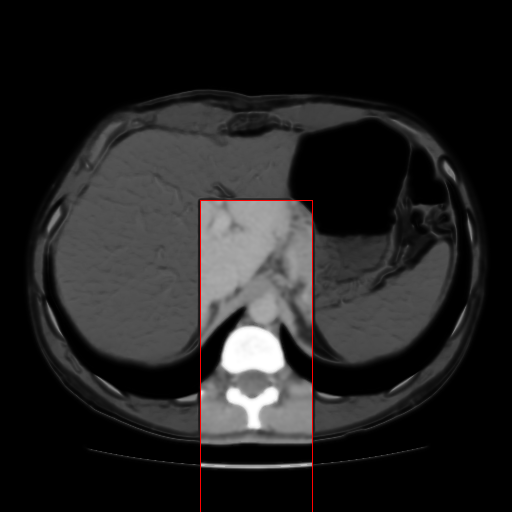
\includegraphics[width=.3\linewidth]{featureid/featureid-2d-spineidentification-seedfinding-a.png}}%
	%
	\hspace{4mm}%
	%
	\subfigure[An example layer $1$ spine seed]
	{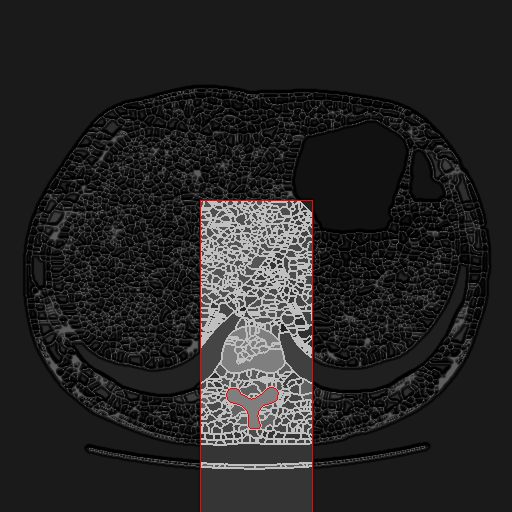
\includegraphics[width=.3\linewidth]{featureid/featureid-2d-spineidentification-seedfinding-b.png}}%
	%
	\hspace{4mm}%
	%
	\subfigure[An example layer $2$ spine seed]
	{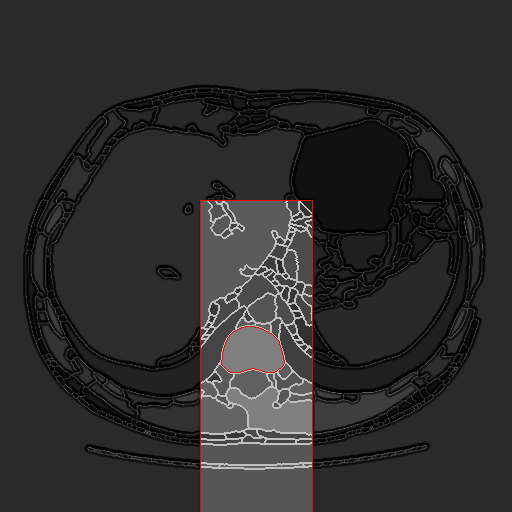
\includegraphics[width=.3\linewidth]{featureid/featureid-2d-spineidentification-seedfinding-c.png}}%
\caption{Finding suitable spine seeds: it suffices to look for moderately-sized, bright regions with centroids within the box shown (this originally appeared as Figure $3$ in \cite{gvcispa09})}
\label{fig:featureid-2d-spineidentification-seedfinding}
\end{stusubfig}
%---

%~~~~~~~~~~~~~~~~~~~~~~~~~~~~~~~~~~~~~~~~~~~~~~~~
\subsubsection{Region Growing}
%~~~~~~~~~~~~~~~~~~~~~~~~~~~~~~~~~~~~~~~~~~~~~~~~

The stratified region growing method itself has already been described in detail above, but it remains to define a suitable \emph{flooding criterion} to decide whether to add an adjacent region to a partial spine being grown from a particular seed, and a \emph{validation criterion} to decide whether to later add that partial spine to the final selection. The flooding criterion I defined in \cite{gvcispa09}, which is specific to $512 \times 512$ images, specifies that an adjacent region should be added if:
%
\begin{itemize}

\item It is at least relatively bright (mean grey value $> 170$)
\item Its centroid $(x,y)$ satisfies $200 \le x \le 312$ and $y \ge 256$

\end{itemize}
%
In this, the threshold for the mean grey value is slightly lower than it was when identifying the spine seeds -- the intuition is that a partial spine should contain at least some regions which are very bright (the seeds), but its mean grey value overall might be lower (this allows pieces of the spine that are more grey than white to be identified by the algorithm).

The validation criterion for partial spines merely ensures that the centroid $(x,y)$ of the partial spine as a whole satisfies $200 \le x \le 312$ and $y \ge 256$.

%~~~~~~~~~~~~~~~~~~~~~~~~~~~~~~~~~~~~~~~~~~~~~~~~
\subsubsection{Post-Processing}
%~~~~~~~~~~~~~~~~~~~~~~~~~~~~~~~~~~~~~~~~~~~~~~~~

Although the stratified region growing process tends to output a preliminary spine that is close to the desired result, it sometimes inadvertently adds regions that should not be part of the spine. Two of the major causes of this are that:
%
\begin{enumerate}

\item By performing flooding in multiple layers, we can end up adding large regions with a high mean grey value that contain smaller regions whose own mean grey value is lower (i.e.~the higher-level regions contain some regions that are spine, and some that aren't).

\item In order to capture greyer bits of the spine, it is necessary to set the mean grey value tolerance in the flooding criterion to a relatively low value (so we end up flooding out into surrounding features such as the aorta, whose mean grey values are above the low threshold).

\end{enumerate}
%
To deal with these problems, it is necessary to post-process the preliminary feature to remove the regions that should not have been added. To do this, we start at each of the nodes in the representation of the preliminary feature, and check whether it should be removed using a \emph{removal criterion} (described shortly). If so, it is removed and the algorithm continues on to the next node in the representation; if not, the algorithm recurses onto the node's branch node children (if any) and applies the same criterion to them. (Note that, although it is not done here, this process could be readily parallelized if desired, since the subtrees beneath each of the nodes in the representation are mutually independent.)

The removal criterion was formulated as a disjunction of two different cases, one to deal with each of the problems mentioned above. The first problem can be dealt with by removing dark regions (those with a mean grey value $< 150$) of a reasonable size (area $\ge 400$). The second problem can be tackled by removing regions that resemble the aorta by having a cross-sectional area between $400$ and $700$ pixels (inclusive), a mean grey value between $160$ and $180$ (inclusive) and an elongatedness $< 1.5$ (since the aorta appears roughly circular in the axial slices being considered).

%~~~~~~~~~~~~~~~~~~~~~~~~~~~~~~~~~~~~~~~~~~~~~~~~
\subsubsection{Results}
%~~~~~~~~~~~~~~~~~~~~~~~~~~~~~~~~~~~~~~~~~~~~~~~~

In terms of results, a qualitative assessment of the identifier conducted for \cite{gvcispa09} proved encouraging -- as described there, I tested the identifier on images from $7$ different series, with results that correlated well with the manual segmentation I would have drawn by hand in the overwhelming majority ($> 85\%$) of cases (some examples are shown in Figure~\ref{fig:featureid-2d-spineidentification-results}). The identifier does still fail in some cases: in particular, this tends to happen when either the spine is significantly darker than usual (e.g.~see case MC-2-135 in the figure) or where there are small pieces of spine that are not connected to the primary feature (e.g.~see cases MC-2-136 and MC-2-137). However, as implemented in the \emph{centipede} system, these cases can be readily corrected by the user, since the identification result is represented as a partition forest multi-feature selection.

%---
\stufigex{height=11cm}{featureid/featureid-2d-spineidentification-results.png}{Results of the 2D spine identification algorithm on images from four different series (BT-2, EJ-2, MC-2 and SD-2): each sub-region is surrounded by its own red border, thus double-thickness borders indicate an internal boundary rather than the boundary of the feature (this originally appeared as Figure $5$ in \cite{gvcispa09})}{fig:featureid-2d-spineidentification-results}{p}
%---

%---
\begin{landscape}
\stufigex{height=.5\linewidth}{featureid/featureid-2d-spineidentification.png}{A graphical overview of the 2D spine identification process (this originally appeared as Figure $4$ in \cite{gvcispa09})}{fig:featureid-2d-spineidentification}{p}
\end{landscape}
%---

\afterpage{\clearpage}
\newpage

%##################################################################################################
\section{Feature Identification in 3D Volumes}
%##################################################################################################

%################################################
\subsection{Overview}
%################################################

Whilst identifying features in 2D can be made to work well much of the time, as was seen in the previous section, such an approach fails to take advantage of important information that is available in adjacent image slices. This can be particularly problematic at the extremities of particular features, or when the cross-section through a feature in a particular slice is not very well distinguished from surrounding tissue. For example, we might not be able to confidently identify a small region as being the right kidney when we can only see the slice in which it lies (see Figure~\ref{fig:featureid-3d-advantage}(a)), but we could be substantially more confident about doing so if we could see the slice below it (see Figure~\ref{fig:featureid-3d-advantage}(b)).

%---
\begin{stusubfig}{p}
	\subfigure[A slice in which the right kidney is hard to see]
	{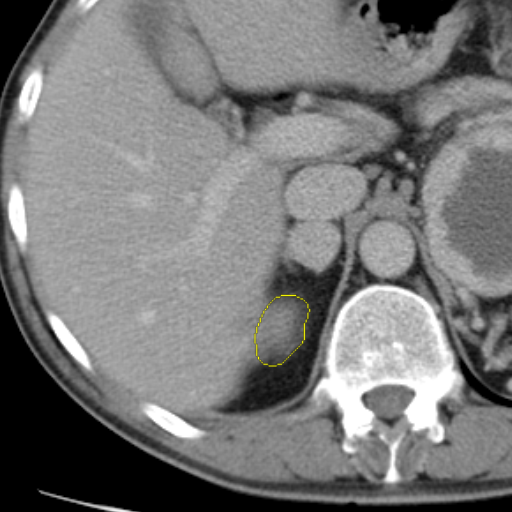
\includegraphics[width=.45\linewidth]{featureid/featureid-3d-advantage-a.png}}%
	%
	\hspace{4mm}%
	%
	\subfigure[The slice below, in which it is obvious]
	{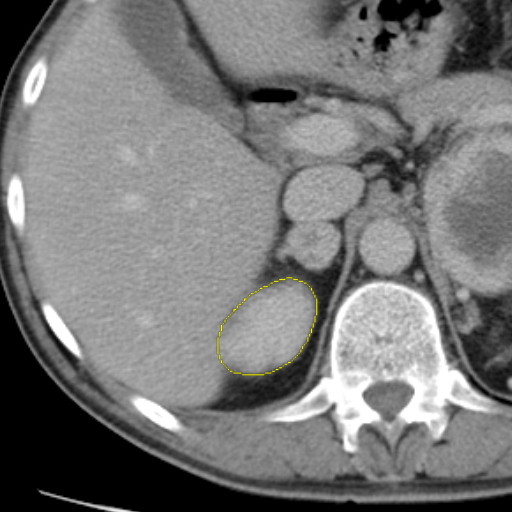
\includegraphics[width=.45\linewidth]{featureid/featureid-3d-advantage-b.png}}%
\caption{We can identify features with much more confidence if we know where they lie in adjacent slices -- but this is difficult to do if we only work with one slice at a time}
\label{fig:featureid-3d-advantage}
\end{stusubfig}
%---

%---
\stufigex{width=.95\linewidth}{featureid/featureid-3d-multifeatureidentifier.png}{The structure of the multi-feature identifier, with dependencies between individual 3D feature identifiers shown as arrows pointing from the identifiers that are run earlier in the identification process to those that depend on them}{fig:featureid-3d-multifeatureidentifier}{p}
%---

Whilst there is more than one way of taking such information into account (for instance, it is possible to imagine a scheme whereby the feature outline from one slice could be propagated to the next slice and deformed to fit the information in the new image), one of the cleanest ways of doing so is to construct a partition forest for the entire 3D CT volume (as described in Chapter~\ref{chap:segmentation}) and then construct new feature identifiers that work in 3D. Using this approach, information from adjacent slices is implicitly taken into account when segmenting the volume into 3D regions.

In this section, therefore, I present a series of methods for identifying a number of 3D features in such a partition forest. Unlike the 2D identifiers presented previously, the 3D identifiers described here are not mutually independent (thus it is not always possible to take an individual identifier out of context and use it to identify its specific feature). Instead, easily-identified features are found first, and then used to identify features that are harder to extract. For example, once the spine (a major landmark) has been identified, it becomes substantially easier to extract the spinal canal (we can intuitively think of it as the darker region inside the spine). As we will see later, it is also possible to use later identifiers to correct any mistakes made by earlier ones. Figure~\ref{fig:featureid-3d-multifeatureidentifier} shows how the identifiers fit together to form a multi-feature identifier.

%################################################
\subsection{Spine Identification}
%################################################

The first 3D feature to identify is the spine. This is an important landmark, both because it is rigid (being made of bone, it does not move within the body when the patient's position changes) and because it is clearly visible in the CT images, even to an untrained eye. It is extremely useful for \emph{localizing} (specifying the position of) other features: for instance, a helpful intuition when identifying the aorta will be that it is roughly located just in front of the spine (i.e.~just above it in the axial slices).

Because the spine is so easily distinguishable in the images, a simple branch node filtering approach is generally sufficient to identify it (if desired, the region(s) thus found can be treated as the seed(s) for a stratified region growing process, but for my purposes this did not prove necessary). A number of criteria are used to isolate the spine (see the pseudo-code in Listing~\ref{code:featureid-3d-spineidentification}), namely that spine regions must:
%
\begin{itemize}

\item Straddle the centre of the image in the $x$ direction.
\item Be at least partially below the centre of the image in the $y$ direction.
\item Extend through all the (axial) slices in the $z$ direction.
\item Have a reasonable $x$-$y$ \emph{aspect ratio} -- i.e.~neither the $x$ nor $y$ dimension of the region's bounding box must be greater than $4$ times the other.
\item Have a mean grey value $\ge 180$.
\item Have a voxel count of between $800$ and $8000$ voxels per (axial) slice.

\end{itemize}
%
Of these, perhaps the most powerful is the criterion that the spine must appear in every slice -- this is particularly effective when there are a significant number of slices in the 3D volume, because very few regions do so, and, in combination with the grey value criterion, more or less prevents false positives. However, it must be applied with an awareness of the scans' location in the body: it would clearly not be appropriate to use such a criterion when viewing scans that go up or down as far as the head or legs.

%---
\begin{stulisting}[t]
\caption{Spine Identification in 3D}
\label{code:featureid-3d-spineidentification}
\lstinputlisting[style=Default]{featureid/featureid-3d-spineidentification.lst}
\end{stulisting}
%---

As the spine identifier has no dependencies on other identifiers, it can be run individually on the CT volume to extract the spine feature. The results of running it on volumes from several different patients, as visualized in Figure~\ref{fig:featureid-3d-spineidentification-results}, give an indication that it works fairly robustly across a wide range of image series; its accuracy will be quantified in Chapter~\ref{chap:validation}. When the identifier is run in isolation, the identified spine tends to also include the spinal canal, as no attempt has thus far been made to exclude it. When identifying multiple features, however, this is later rectified by the spinal canal identifier, which unmarks any regions incorrectly labelled as spine where necessary. The identified spine can sometimes also include pieces of rib where they join onto the spinal column; the current approach to rib identification does not handle this at present, but it is an interesting area for further work.

%---
\begin{stusubfig}{p}
	\subfigure[Series BT-2 (Slices 60--80)]
	{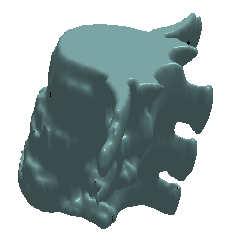
\includegraphics[height=6cm]{featureid/featureid-3d-spineidentification-BT-2-60-80.png}}%
	%
	\hspace{4mm}%
	%
	\subfigure[Series SD-2 (Slices 70--90)]
	{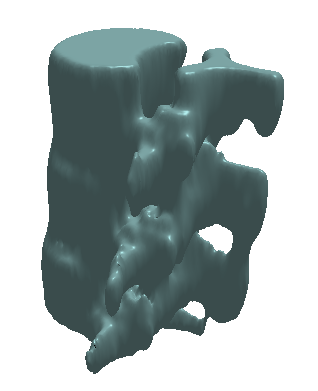
\includegraphics[height=6cm]{featureid/featureid-3d-spineidentification-SD-2-70-90.png}}%
	%
	\\
	%
	\subfigure[Series MC-2 (Slices 110--130)]
	{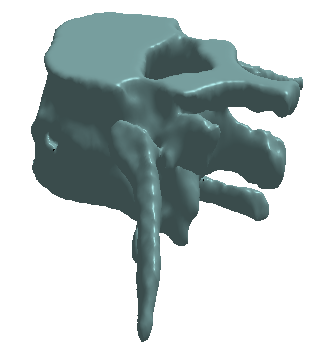
\includegraphics[height=6cm]{featureid/featureid-3d-spineidentification-MC-2-110-130.png}}%
	%
	\hspace{4mm}%
	%
	\subfigure[Series EJ-2 (Slices 20--40)]
	{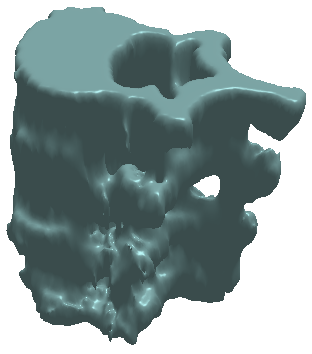
\includegraphics[height=6cm]{featureid/featureid-3d-spineidentification-EJ-2-20-40.png}}%
	%
	\\
	%
	\subfigure[Series MJ-2 (Slices 110--130)]
	{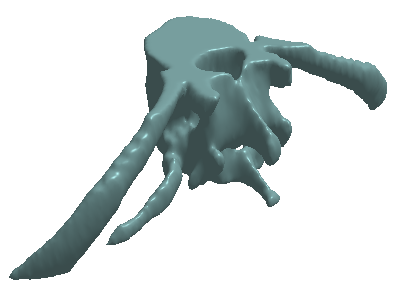
\includegraphics[height=6cm]{featureid/featureid-3d-spineidentification-MJ-2-110-130.png}}%
	%
	\hspace{4mm}%
	%
	\subfigure[Series EB-2 (Slices 60--80)]
	{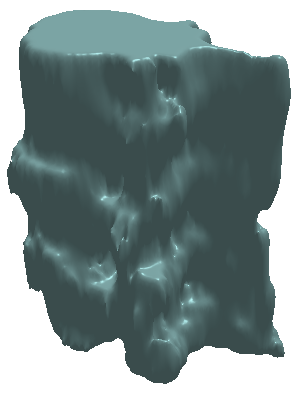
\includegraphics[height=6cm]{featureid/featureid-3d-spineidentification-EB-2-60-80.png}}%
\caption{The results of running the spine identifier in isolation on slices from six different image series}
\label{fig:featureid-3d-spineidentification-results}
\end{stusubfig}
%---

\afterpage{\clearpage}
\newpage

%################################################
\subsection{Spinal Canal Identification}
%################################################

%---
\stufigex{height=9cm}{featureid/featureid-3d-spinalcanalidentification-region.png}{The spinal canal (selected, in red) should lie well within the (yellow) bounding box of the regions identified as the spine}{fig:featureid-3d-spinalcanalidentification-region}{h}
%---

\noindent Having first identified the spine, identifying the spinal canal becomes a much simpler task. The intuition is to search for regions well within the $x-y$ bounding box of the spine (see Figure~\ref{fig:featureid-3d-spinalcanalidentification-region}) that:
%
\begin{itemize}

\item Straddle the spine centroid in the $x$ direction.
\item Extend through all the (axial) slices in the $z$ direction (this could be alternatively phrased as `appear in every slice in which the spine does', if a more sophisticated approach to spine identification was being used).
\item Have a mean grey value $\le 140$ (the spinal canal appears much darker on the CT scans than the vertebrae surrounding it).
\item Have a voxel count of between $300$ and $1000$ voxels per (axial) slice.

\end{itemize}
%
Regions which satisfy these criteria are unmarked as spine (if necessary) and marked as spinal canal. Unlike the spine identifier, the spinal canal identifier clearly cannot be run in isolation, but it is possible to visualize the results of spinal canal identification by running both the spine and spinal canal identifiers and then either rendering the spinal canal on its own, or rendering the spine as transparent. As illustrated in Figure~\ref{fig:featureid-3d-spinalcanalidentification-results}, the identifier is quite robust, and able to automatically identify the spinal canal in a number of different image series. There is, however, definitely room for further work to improve the detailed contour of the canal -- this could perhaps be done by using the automatic result produced thus far to initialise a level sets approach.

%---
\begin{stulisting}[!b]
\caption{Spinal Canal Identification in 3D}
\label{code:featureid-3d-spinalcanalidentification}
\lstinputlisting[style=Default]{featureid/featureid-3d-spinalcanalidentification.lst}
\end{stulisting}
%---

%---
\begin{stusubfig}{p}
	\subfigure[Series BT-2 (Slices 60--80), Spine and Spinal Canal]
	{\hspace{8mm}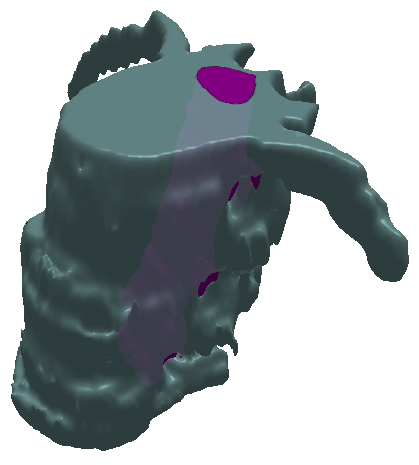
\includegraphics[height=6cm]{featureid/featureid-3d-spinalcanalidentification-transparent-BT-2-60-80.png}\hspace{8mm}}%
	%
	\hspace{4mm}%
	%
	\subfigure[Series BT-2 (Slices 60--80), Spinal Canal Only]
	{\hspace{12mm}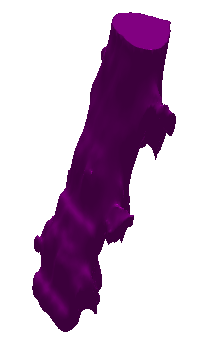
\includegraphics[height=6cm]{featureid/featureid-3d-spinalcanalidentification-solid-BT-2-60-80.png}\hspace{12mm}}%
	%
	\\
	%
	\subfigure[Series SD-2 (Slices 70--90), Spine and Spinal Canal]
	{\hspace{16mm}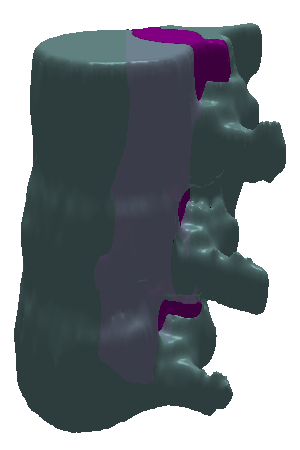
\includegraphics[height=6cm]{featureid/featureid-3d-spinalcanalidentification-transparent-SD-2-70-90.png}\hspace{16mm}}%
	%
	\hspace{4mm}%
	%
	\subfigure[Series SD-2 (Slices 70--90), Spinal Canal Only]
	{\hspace{20mm}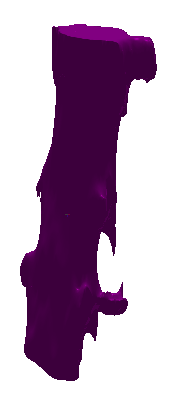
\includegraphics[height=6cm]{featureid/featureid-3d-spinalcanalidentification-solid-SD-2-70-90.png}\hspace{20mm}}%
	%
	\\
	%
	\subfigure[Series EJ-2 (Slices 20--40), Spine and Spinal Canal]
	{\hspace{12mm}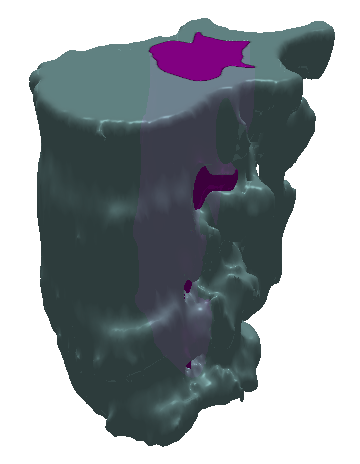
\includegraphics[height=6cm]{featureid/featureid-3d-spinalcanalidentification-transparent-EJ-2-20-40.png}\hspace{12mm}}%
	%
	\hspace{4mm}%
	%
	\subfigure[Series EJ-2 (Slices 20--40), Spinal Canal Only]
	{\hspace{20mm}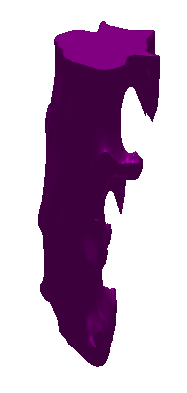
\includegraphics[height=6cm]{featureid/featureid-3d-spinalcanalidentification-solid-EJ-2-20-40.png}\hspace{20mm}}%
\caption{The results of running spine and spinal canal identification on slices from three different image series}
\label{fig:featureid-3d-spinalcanalidentification-results}
\end{stusubfig}
%---

\afterpage{\clearpage}
\newpage

%################################################
\subsection{Ribs Identification}
\label{subsec:featureid-3d-ribsidentification}
%################################################

%---
\stufigex{height=9cm}{featureid/featureid-3d-ribsidentification-region}{The spatial constraints for rib seeds -- they must be at least partly in one of the regions labelled `R', and no part of them must lie in the region labelled `T'}{fig:featureid-3d-ribsidentification-region}{h}
%---

\noindent In contrast to the spine and spinal canal identifiers, which can (at least to a first approximation) often identify their features using only branch node filtering, the 3D ribs identifier is necessarily more involved, because it is unusual for each rib to be represented by only a single node in the forest. For that reason, a stratified region growing method is preferred in this case, followed by customised post-processing to tidy up the results. The first step is to identify suitable seeds for the ribs, namely regions that:
%
\begin{itemize}

\item Are relatively small, having a voxel count of less than $500$ voxels per slice.
\item Have a high mean grey value $\ge 200$.
\item Do not extend significantly below the spine (this helps to exclude pieces of the table on which the patient is lying, which might otherwise look quite rib-like).
\item Are not completely contained within the spine's bounding box in the $x$ axis.

\end{itemize}
%
The spatial constraints are illustrated in Figure~\ref{fig:featureid-3d-ribsidentification-region}. Having found suitable seeds, the next step is to grow regions from them, using the grow condition that we should flood into an adjacent region iff its mean grey value is $\ge 180$ and it is not already marked as spine. Setting the mean grey value threshold slightly lower than that required for seeds makes it possible to identify ribs that are slightly grey in places. Excluding the spine is done to prevent ribs growing into the spine, since they are attached to the spinal column. As mentioned when describing the spine identifier, the identifiers do not currently manage to perfectly separate the spine and ribs -- the current approach effectively assigns pieces to the spine when in doubt. This is a suitable area for further work.

The final step is to post-process the results of the stratified region growing process, which at this point in the algorithm are represented as a partition forest selection. As the post-processing involves connected component analysis, the selection must first be viewed at the level of the selected nodes' \emph{merge layer} (so called because it is the layer in which the nodes would be merged), namely the lowest layer containing a selected node. We will call the nodes \emph{viewed nodes} when viewed at this level. Of these viewed nodes, we remove any that are too dark to be part of the aorta -- specified as having a mean grey value $< 150$. We then find the connected components of the remaining viewed nodes, after which each connected component has its voxel count compared to minimum and maximum thresholds. Connected components that meet the size requirements are added to the final result, whilst the remainder are discarded.

As illustrated in Figure~\ref{fig:featureid-3d-ribsidentification-results}, this identification process has been used to produce satisfactory (if not perfect) results on images from a number of different series. However, it needs further refinement to make it more robust. Two specific issues to be addressed in further work are that some of the ribs can be inadvertently captured by the spine, since the features are connected and share similar grey value distributions, and that some of the hard size constraints can cause ribs to be missed when they are too large or too small. The accuracy of the identifier in cases where it does and does not work well will be evaluated in the next chapter.

%---
\begin{stulisting}[p]
\caption{Ribs Identification in 3D}
\label{code:featureid-3d-ribsidentification}
\lstinputlisting[style=Default]{featureid/featureid-3d-ribsidentification.lst}
\end{stulisting}
%---

%---
\begin{stusubfig}{p}
	\subfigure[Series BT-2 (Slices 60--80)]
	{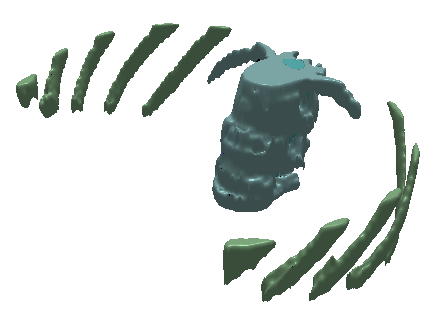
\includegraphics[width=.45\linewidth]{featureid/featureid-3d-ribsidentification-BT-2-60-80.png}}%
	%
	\hspace{4mm}%
	%
	\subfigure[Series SD-2 (Slices 50--70)]
	{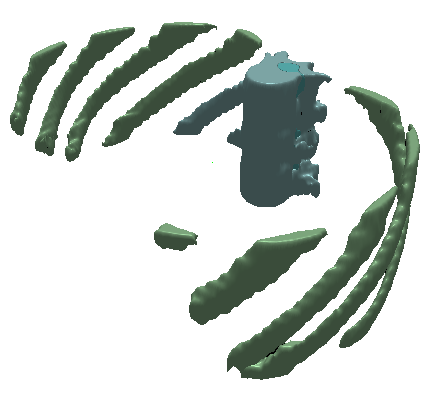
\includegraphics[width=.45\linewidth]{featureid/featureid-3d-ribsidentification-SD-2-50-70.png}}%
	%
	\\
	%
	\subfigure[Series MC-2 (Slices 80--100)]
	{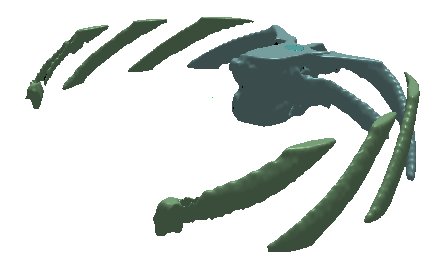
\includegraphics[width=.45\linewidth]{featureid/featureid-3d-ribsidentification-MC-2-80-100.png}}%
	%
	\hspace{4mm}%
	%
	\subfigure[Series EJ-2 (Slices 1--21)]
	{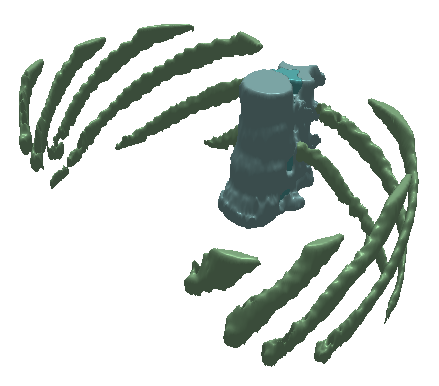
\includegraphics[width=.45\linewidth]{featureid/featureid-3d-ribsidentification-EJ-2-1-21.png}}%
\caption{The results of running spine, spinal canal and ribs identification on slices from four different image series}
\label{fig:featureid-3d-ribsidentification-results}
\end{stusubfig}
%---

\afterpage{\clearpage}
\newpage

%################################################
\subsection{Aorta Identification}
%################################################

TODO

%---
\begin{stulisting}[p]
\caption{Aorta Identification in 3D}
\label{code:featureid-3d-aortaidentification}
\lstinputlisting[style=Default]{featureid/featureid-3d-aortaidentification.lst}
\end{stulisting}
%---

%---
\begin{stusubfig}{p}
	\subfigure[Series BT-2 (Slices 60--80)]
	{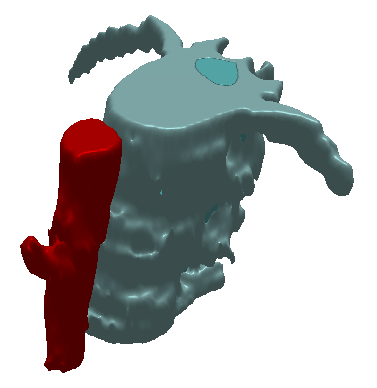
\includegraphics[height=6cm]{featureid/featureid-3d-aortaidentification-BT-2-60-80.png}}%
	%
	\\
	%
	\subfigure[Series SD-2 (Slices 60--80)]
	{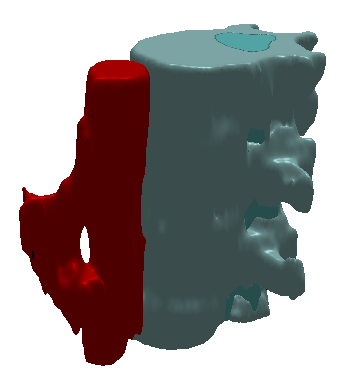
\includegraphics[height=6cm]{featureid/featureid-3d-aortaidentification-SD-2-60-80.png}}%
	%
	\\
	%
	\subfigure[Series EJ-2 (Slices 10--30)]
	{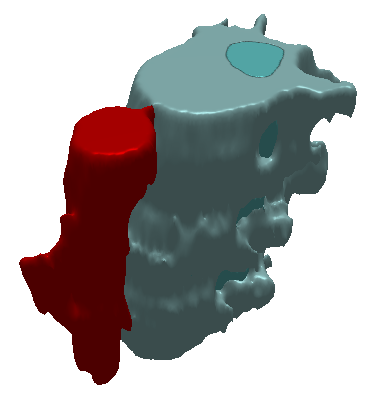
\includegraphics[height=6cm]{featureid/featureid-3d-aortaidentification-EJ-2-10-30.png}}%
\caption{The results of running spine, spinal canal and aorta identification on slices from three different image series}
\label{fig:featureid-3d-aortaidentification-results}
\end{stusubfig}
%---

\afterpage{\clearpage}
\newpage

%################################################
\subsection{Liver Identification}
%################################################

TODO

%---
\begin{stulisting}[p]
\caption{Liver Identification in 3D}
\label{code:featureid-3d-liveridentification}
\lstinputlisting[style=Default]{featureid/featureid-3d-liveridentification.lst}
\end{stulisting}
%---

\afterpage{\clearpage}
\newpage

%################################################
\subsection{Kidneys Identification}
%################################################

TODO (remember to mention that non-complete kidneys, e.g.~those with tumours on, are particularly vulnerable to being missed -- an example is the EB result, where one kidney has been perfectly identified and the other has been completely missed)

%---
\begin{stulisting}[p]
\caption{Kidneys Identification in 3D}
\label{code:featureid-3d-kidneysidentification}
\lstinputlisting[style=Default]{featureid/featureid-3d-kidneysidentification.lst}
\end{stulisting}
%---

%---
\begin{stusubfig}{p}
	\subfigure[Series BT-2 (Slices 59--81)]
	{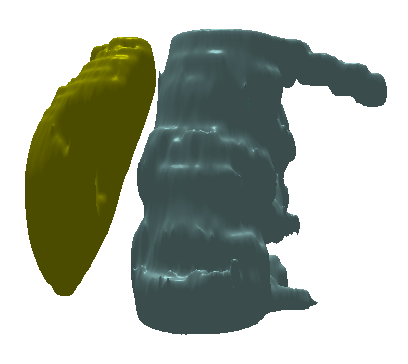
\includegraphics[height=6cm]{featureid/featureid-3d-kidneysidentification-BT-2-59-81.png}}%
	%
	\hspace{4mm}%
	%
	\subfigure[Series SD-2 (Slices 69--90)]
	{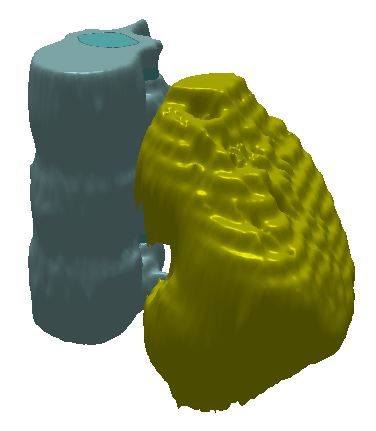
\includegraphics[height=6cm]{featureid/featureid-3d-kidneysidentification-SD-2-69-90.png}}%
	%
	\\
	%
	\subfigure[Series KB-2 (Slices 76--100)]
	{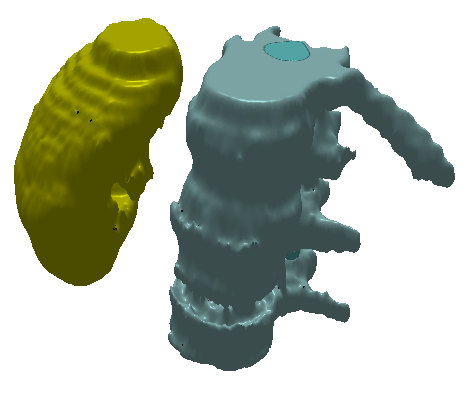
\includegraphics[height=6cm]{featureid/featureid-3d-kidneysidentification-KB-2-76-100.png}}%
	%
	\hspace{4mm}%
	%
	\subfigure[Series EB-2 (Slices 59--80)]
	{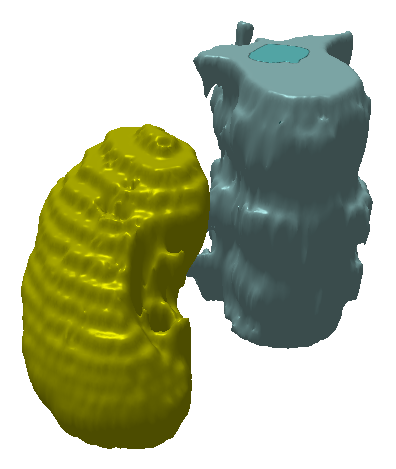
\includegraphics[height=6cm]{featureid/featureid-3d-kidneysidentification-EB-2-59-80.png}}%
	%
	\\
	%
	\subfigure[Series EJ-2 (Slices 16--40)]
	{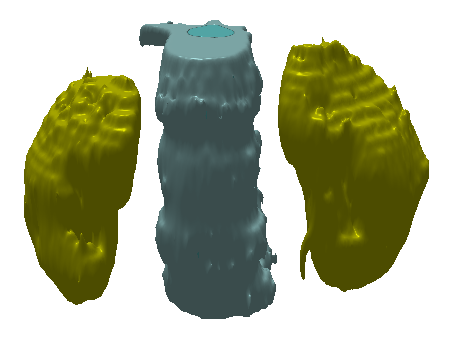
\includegraphics[height=6cm]{featureid/featureid-3d-kidneysidentification-EJ-2-16-40.png}}%
\caption{The results of running spine, spinal canal and kidney identification on slices from five different image series}
\label{fig:featureid-3d-kidneysidentification-results}
\end{stusubfig}
%---

\afterpage{\clearpage}
\newpage

%################################################
\subsection{Results}
%################################################

TODO: Limited results, as proper validation will be done in the following chapter

%##################################################################################################
\section{Chapter Summary}
%##################################################################################################

TODO
